\chapter{Clustering}
\emph{Clustering} analysis relate to finding groups of objects such that the objects in a group will be similar (or related) to one another 
and different from (or unrelated to) the objects in other groups, as it is possible to note in figure \ref{img:cluster}

\begin{figure}
    \caption{Cluster Example}
    \label{img:cluster}
    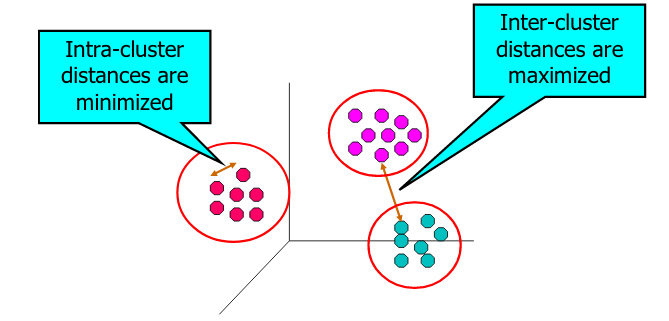
\includegraphics[width=\textwidth]{Images/cluster}
\end{figure}

\begin{figure}
    \caption{Ambiguity about number of Cluster}
    \label{img:ambiguousCluster}
    \includegraphics[width=\textwidth]{Images/ambiguousCluster}
\end{figure}

The notion of cluster can be ambiguous as can be note in figure \ref{img:ambiguousCluster} and a clustering is a set of clusters, where exist
an important distinction between:
\begin{description}
    \item [Partitional Clustering: ] a division of data objects into non-overlapping subsets (clusters) such that each data object is in exactly one subset
    				     as can be viewed in figure \ref{img:partitionalCluster}.

				     \begin{figure}
				         \caption{Example of Partitional Clustering}
					 \label{img:partitionalCluster}
					 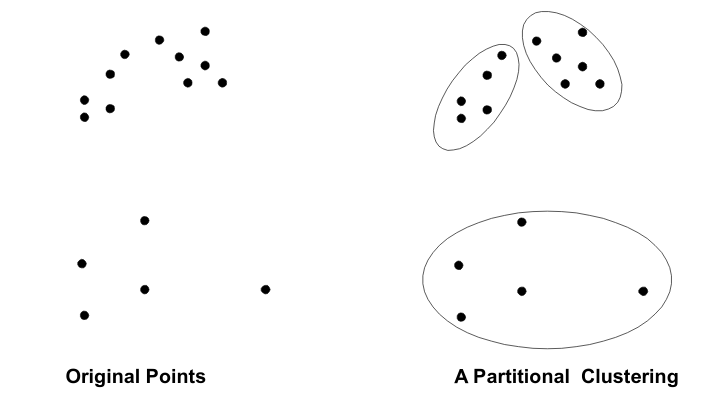
\includegraphics[width=\textwidth]{Images/partitional}
				     \end{figure}

    \item [Hierarchical Clustering: ] a set of nested clusters organized as a hierarchical tree, as can be note in figure \ref{img:hierarchicalCluster}.

    				      \begin{figure}
				          \caption{Example of Hierarchical Clustering}
					  \label{img:hierarchicalCluster}
					  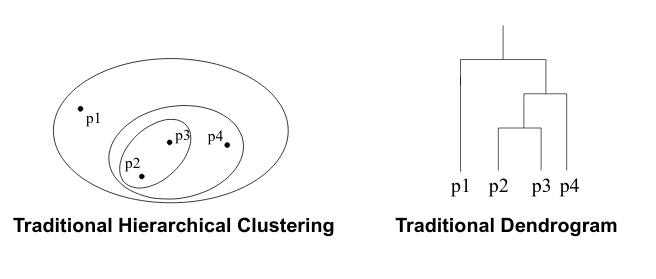
\includegraphics[width=\textwidth]{Images/hierarchical}
				      \end{figure}
\end{description}
ARRIVE UNTIL SLIDE 16


